\documentclass[12pt]{article}

\usepackage[T1]{fontenc} 
\usepackage[utf8]{inputenc}
\usepackage[francais]{babel}
\usepackage{graphicx}
\usepackage{hyperref}
\usepackage{url}
\usepackage{color}
\usepackage[usenames,dvipsnames]{xcolor}
\usepackage{alltt}
\usepackage{tocbibind}


\title{Rapport Final projet EDD}
\author{Pinero, Borde, Bonnet}

\begin{document}
\maketitle
\tableofcontents

\newpage

\section{Le projet}
\subsection{Présentation}
Le projet se compose de plusieurs parties de développement sur un sujet
commun, le jeu du 2048. Ce jeu consiste à additionner des tuiles de même
puissance de 2, sur un plateau de 16 tuiles, jusqu'à ce que le plateau soit
plein et qu'aucune addition ne soit possible. Le but du jeu est d’arriver \'a
construire une brique de valeur la plus grande possible (2048, 4096,
8192, \ldots)

\subsection{Le sujet}
Dans le projet nous avons eu à réaliser dans un premier temps l'ensemble du
moteur du jeu et quelques tests qui nous garantissent au maximum la solidité de notre code 
pendant le développement. Dans un deuxième temps, nous devions faire la
" critique " du développement de la première partie faite par
d'autres groupes basé sur une grille d'évaluation qui nous a été
fournie. Ensuite nous avons réalisé un ensemble de stratégies de jeu qui
sont capables de jouer de manière autonome une partie entière. Ces stratégies doivent à chaque tour calculer le meilleur
prochain coup pour atteindre le plus grand score possible. La dernière partie
du projet consiste à réaliser une véritable interface graphique pour
jouer au jeu.

\newpage
\section{Développement du 2048 et tests}
Pour le développement du 2048, le langage de programmation était imposé,
nous devions utiliser le langage C. Chaque groupe a dû fournir les sources
permettant de générer une bibliothèque libgrid.a (implémentant les
fonctions décrites dans grid.h en annexe \ref{grid_h}) ainsi qu’un
exécutable permettant de jouer au 2048 dans la console. En plus de ça, nous
avons réalisé des tests pour vérifier toutes les fonctions
implémentées.\par

Avant de commencer le travail de développement, nous avons utilisé un
outil de gestion de versions décentralisé pour que chaque membre du groupe
puisse avoir accès à chaque instant à la dernière version du projet.
Pour ça nous avons choisi le logiciel \href{http://git-scm.com/}{GIT}, et la plateforme
\href{http://github.com/}{GitHub}. Les sources du projet ont été disponibles tout
au long du développement \href{http://github.com/kamneo/EDD_project}{ici}.\par

En ce qui concerne l'arborescence de notre projet, nous avons décidé d'avoir
une organisation bien précise pour qu'elle puisse être le plus générique et le plus modulable possible
, c'est-\`a-dire qu'elle s'adapte aux évolutions du projet ou au modification de constante tel que la taille.
Mais surtout pour qu'elle soit la plus clair possible.

\begin{alltt}
{\color{gray}
EDD_projet/        # Racine du projet
    bin/           # Fichiers exécutables.
    build/         # Fichiers de compilation du projet
    include/       # Fichiers .h des librairies générées
    lib/           # Librairies
    src/           # Fichiers sources
        2048/      # Fichiers sources de l'interface graphique
        grid/      # Fichiers du moteur de jeu
            tests/ # Fichiers qui testent le moteur de jeu
}
\end{alltt}

\par

Tout au long du développement du projet, tous les membres du groupe se sont
mis d'accord sur le fait d'utiliser l'outil \href{http://www.cmake.org/}{CMake}
pour compiler le projet, générer les Makefiles qui servent eux-mêmes à générer
les exécutables, les librairies et exécuter les tests.

\subsection{Le développement de grid.c}
En ce qui concerne le développement de grid.c, qui est le moteur du jeu,
c'était relativement simple. Les fonctions qui ont mérité une réflexion
sérieuse sont " do\_move() " et " can\_move() ". Pour ces
fonctions nous devions limiter au mieux la duplication de code et la complexité
de l'algorithme. Chose que nous n'avions au final pas très bien r\'eussi, mais
nous verrons dans la partie \ref{notre_etude}.

\subsubsection{Implémentation de " can\_move "}
Pour cette fonction, nous avons choisi l'algorithme suivant :

\begin{alltt}
{\color{gray}
Si la direction donnée est " UP " ou " DOWN " alors
    Pour chaque colonne faire :
        Pour chaque tuile de la colonne faire :
            Si la tuile précédente est égale à la courante
                retourner vrai
 		
            Si la tuile courante est non vide 
                   et qu'il y a une tuile vide dans la colonne
                retourner vrai	    	
Si la direction donnée est " RIGHT " ou " LEFT " alors
    Pour chaque ligne faire 
        Pour chaque tuile de la ligne faire
            Si la tuile précédente est égale à la courante
                retourner vrai
 		
            Si la tuile courante est non vide
                   et qu'il y a une tuile vide dans la ligne
                retourner vrai	    	
retourner faux
}
\end{alltt}

C'est là que l'on peut voir que nous avons commis une erreur nous n'aurions
pas d\^u partir sur un algorithme qui traite séparément les directions haut/bas et droite/gauche.

Cette fonction est utilisée à plusieurs reprises dans d'autres fonctions
comme par exemple " game\_over " ou " do\_move ". d'o\`u
l'importance qu'elle n'ai pas une trop grande complexité de calcul.

\subsubsection{Implémentation de " do\_move "}
Pour cette fonction, nous avons choisi l'algorithme suivant :
\begin{alltt}
{\color{gray}
Si la direction donnée ne peut pas être jouée
    Ne rien faire
     
Si la direction donnée est " UP " ou " DOWN " alors
    Pour chaque colonne faire :
        Pour chaque tuile de la colonne faire :
            Si la tuile précédente est égale à la courante
                On fusionne les deux tuiles
                On modifie le score de la partie
            
            Si la tuile courante est vide alors
            	On change sa place avec la première tuile non vide
            	
Si la direction donnée est " RIGHT " ou " LEFT " alors
    Pour chaque ligne faire 
        Pour chaque tuile de la ligne faire :
            Si la tuile précédente est égale à la courante
                On fusionne les deux tuiles
                On modifie le score de la partie
            
            Si la tuile courante est vide alors
            	On change sa place avec la première tuile non vide
}
\end{alltt}

\subsection{L'affichage de la grille dans la console}
Pour l'affichage de la grille dans la console, nous avons eu plusieurs versions
et designs. La toute première version était une simple grille dans la console
o\`u était affiché le score et les valeurs des tuiles. Dans cette version
nous devions jouer avec les lettres Z, Q, S et D du clavier car dans le langage C, la
fonction " scanf " de la librairie " stdio " qui permet de
lire l'entrée standard, ne prend pas en compte les flèches du clavier.
En annexe vous trouverez une capture d'écran de cette version.\par
Dans une deuxième version, nous avions décidé de mettre des couleurs dans
les tuiles en fonction de leurs valeurs. (à voir en annexe \ref{grille_couleur}).\par
Enfin pour répondre correctement au sujet, nous avons utilisé la librairie
" NCurses ". L'utilisation de cette librairie nous a permis de se
libérer de deux de nos difficultés. La première était que nous devions jouer
avec des lettres et non les flèches du clavier, la seconde était que nous
n'avions pas d'affichage dynamique de la grille à chaque coup. Pour être plus
clair, lorsqu'on jouait un coup avec les deux premières versions de
l'affichage, la grille du coup précédent était toujours présente dans la
console. Désormais, la console n'affiche plus qu'une grille et elle met-à-jour après chaque coup.\par

La version ncurses de notre projet n'a cependant pas été très facile à implémenter.
Ce genre de librairie demande un grand nombre d'initialisations de variables qui rendent
difficile la conservation d'un code propre mais aussi qui multiplie les risques de fuite mémoire.
Nous somme cepandant satisfaits du résultat car a part une toute petite fuite
découverte pendant l'évaluation des autres groupes (corrigé depuis) aucun problème n'a été relevé.

\subsection{Les tests}
Les Tests sont écrits pour confronter une réalisation à sa spécification.
Le test définit un critère d’arrêt (état ou sorties à l’issue de
l’exécution) et permet de statuer sur le succès ou sur l’échec d’une
vérification. Gr\^ace à la spécification, on est en mesure de faire
correspondre un état d’entrée donné à un résultat ou à une sortie.
Le test permet de vérifier que la relation d’entrée / sortie donnée par la
spécification est bel et bien réalisée.
\cite{Test_unitaire}

\par Sur ce principe nous avons réalisé un test par fonction décrite dans
le fichier " grid.h " et un test sur la réalisation de plusieurs parties
qui s'exécutent avec une stratégie basique qui consiste à jouer à gauche
si on le peut sinon à droite, sinon en haut et enfin en bas. Ainsi lorsqu'on fait
des modifications de l'une de ces fonctions, nous nous assurons que cela n'a en
rien changé à la véracité des résultats. L'exécution des tests
s'effectue avec la commande " make test ". L'utilisation de l'outil " CMake " nous permet
d'avoir un affichage complet à la fin des tests sur leurs résultats pour savoir s'ils sont passés avec succès
ou non (exemple en annexe \ref{test}).

\par Comme dit précédemment, chaque test est spécifique à une fonction:
\begin{itemize}
  \item La création d'une grille et son initialisation correcte.
  \item L'homogénéité de la fonction add\_tile, c'est-à-dire que la
  probabilité que la tuile générée soit bien de $
  \frac{1}{le\ nombre\ de\ tuiles} $ avec une marge de 0.05\%.
  \item La véracité des fonctions " game\_over " et " can\_move
  "
  \item La bonne exécution des mouvements dans chaque direction.
  \item Enfin l'exécution sans erreur de 1000 parties.
\end{itemize}

\newpage
\section{Relectures critiques}
à l’issue de la première phase de travail, chaque groupe a dû relire le code produit par trois autres groupes. Pour chaque groupe à relire, on a
rempli un formulaire d’évaluation. Ce formulaire d’évaluation nous a été
fourni par notre chargé de TD.

\par Cette feuille d'évaluation était composée de 13 questions orientées
sur trois axes. Le point de vue utilisateur, qui pousse à vérifier
principalement la propreté de l'archive, que la compilation ne génère pas
d'erreur et qu'il y a un fichier " README " pour expliquer l'utilisation
du programme si ce n'est pas évident. Dans un deuxième temps, d'un point de
vue fonctionnel, nous devions vérifier si le programme ne présente pas de
bogue ou de fuite mémoire. Enfin, d'un point de vue programmation, nous
devions porter notre attention sur les patrons de conception (ou \textit{design
patterns} en anglais).

\subsection{Les relectures que nous avons réalisé}
Nous avons eu à faire la relecture des groupes A, D et G. Comme nous sommes
trois, nous nous sommes divisé le travail et avons évalué un groupe
chacun. Nous nous sommes ensuite concerté pour harmoniser nos commentaires.
Cette relecture fût très intéressante car elle nous a permis de mettre au
premier plan les points importants sur lesquels il faut insister lors du
développement d'un projet. En plus de cela, comme chaque groupe a eu le choix
sur la façon d'implémenter son programme, nous avons vu les différentes
possibilités d'implémentation parfois meilleures et plus efficaces ou pas. Le
but n'était pas d'être trop sévère ou au contraire laxiste sur nos
commentaires (car ceux que nous avons donné sur chaque projet n'ont pas été
notés) mais d'avoir un esprit critique sur le code de nos camarade. Car s'il est plus facile
de juger le travail d'un autre cela finit forcement par remettre en question notre
propre travail.
\subsection{Les relectures réalisées par les autres groupes}
\label{notre_etude}
En ce qui concerne les commentaires qui ont été faits par les autres groupes
sur notre projet, nous les avons trouvés justifiés. Même si, il faut
l'avouer, recevoir des " critiques " sur le travail que nous avons
réalisé pendant près de trois ou quatre semaines n'est pas agréable. Nous avons pris ces critiques
en compte et en avons corrigé un maximum avant le rendu final. 
\par Nous avons principalement reçu des commentaires négatifs sur la
duplication de code dans l'implémentation du moteur de jeu. Certaines fonctions
qui sont utilisées dans les fonctions " can\_move " et " do\_move " se
ressemblent fortement. Un autre point à été remarqué, le nommage des
variables et les commentaires dans le code source étaient certaines fois en
français et d'autre en anglais alors que les patrons de conceptions nous
imposaient de les mettre qu'en anglais. Il restait aussi une petite fuite mémoire
qui nous avait échappé dans ncurses. Hormis la factorisation de do\_move et can\_move tout
est à l'heure actuelle corrigé. Nous n'avons malheureusement pas eu le temps de
reprendre l'implémentation de ces fonctions qui demanderait de reprendre
leur algorithme à zéro ce qui n'est pas évident.

\newpage
\section{Les stratégies}
Dans cette partie, chacun des groupes a dû mettre au point au minimum deux
stratégies. Une stratégie rapide (capable de jouer une partie en moins de
10s) et une stratégie plus gourmande (capable de jouer une partie en moins de
2min). Une stratégie est une structure qui implémente l’interface décrite
dans strategy.h. Chaque stratégie est de la forme d’une bibliothèque
dynamique. Nous avons implémenté quatre stratégies pour l'instant, deux
plutôt triviales qui sont basées sur la stratégie du coin, et deux autres sur
la stratégie " expected max ". 

\subsection{Stratégie du coin}
La stratégie fonctionnelle choisie pour le rapport est la stratégie du coin.
Pour cela, nous avions fait un premier algorithme qui se contente de jouer vers
la gauche tant qu'on le peut, sinon il joue vers le bas encore une fois tant
qu'on le peut, de même vers la droite puis vers le haut. Avec cette stratégie,
sur 48 parties nous avons un score moyen de 2475, avec 6x64, 20x128, 20x256 et
2x512.

Dans un second temps, nous avons fait un second algorithme qui est basé sur le
premier mais qui un coup sur deux change les mouvements favoris. Les premiers
mouvements favoris sont dans cet ordre, gauche, bas, droite et haut, et les
seconds mouvements sont dans cet ordre, bas, gauche, droite et haut. Avec cette
stratégie, sur 48 parties nous avons un score moyen de 2259, avec 1x32, 3x64,
21x128 et 23x256.

Les deux stratégies se valent à peu près, mais c'est bien la première qui est la
meilleure. Bien sûr cette stratégie n'était qu'un essai et ces résultats sont
très mauvais, les vraies stratégies arrivent après.

\subsection{Implémentation d'expected max}
" Expected Max " est un algorithme qui consiste à retourner la direction
optimale à jouer. Elle est basée sur l'algorithme " minimax ". Le
principe est de donner une valeur à la grille en fonction de plusieurs critères
(cf. " \ref{eval_grid} Evaluation de la grille ") ainsi nous jouerons le
coup avec le maximum de chances de gagner combiné au coup avec le minimum de
chances de perdre.
\par L'une des limites de cette méthode est qu'il faille jouer à deux
joueurs, or au 2048 on joue tout seul. C'est pour cette raison qu'on n'utilisera
pas le théorème du " minimax " mais celui d'" expected Max ". En effet
ici on considèrera le second joueur comme l'ordinateur qui remplira de façon
aléatoire une des tuiles vides après la direction choisie. Cela engage de
calculer, pour chaque grille et pour toutes les possibilités de remplissage
d'une tuile vide, la valeur de cette grille. Il faudra ensuite faire une moyenne
de toutes les valeurs calculées pour chaque direction afin de déterminer
laquelle est la plus intéressante. Pour un algorithme encore plus performant il serait
avantageux de pouvoir étendre notre arbre à une profondeur N choisie au
début du programme. Il parait évident qu'une telle technique va avoir un coût
en mémoire et calcule important. Hors dans la mesure où des limitations en temps
d'exécution nous sont imposées il faudra trouver un équilibre entre résultats et
performances.
\par Pour la stratégie courte nous n'allons qu'à une profondeur de 2 (nous
avons deux sous arbres) et calculons avec une probabilité de 100 \%
d'avoir une tuile de valeur 2 qui apparait. Pour la stratégie plus
efficace, nous allons à une profondeur de trois et nous prenons en compte
la probabilité de 10 \% qu'il y ai une tuile de valeur 4 qui soit
générée.

\subsection{Evaluation de la grille}
\label{eval_grid}
Pour évaluer la grille, nous avons pris en compte quatre paramètres, et à chacun
de ces paramètres nous leurs avons donné un coefficient pour leur donner plus ou
moins d'importance. \cite{Eval}

\subsubsection{Le nombre de tuiles vides}
On compte le nombre de tuiles vides que l'on a après avoir joué.
\subsubsection{La plus grande tuile} 
Est la valeur de la tuile avec la plus grande valeur.

\subsubsection{La grille la plus progressive possible}
Une grille est progressive lorsque la valeur des cases augmente ou descend
quelle que soit la direction. Ainsi, 2 - 4 - 8 - 16 est acceptable, tout comme
32 - 8 - 4 - 2. Mais 2 - 8 - 2 - 16 ne l'est pas (à cause de la 3eme case).
\`A chaque mouvement on doit vérifier si  le mouvement d'après rendra la
grille plus progressive. Si c'est le cas, le mouvement doit être effectué.
Si non, trouver un autre mouvement.

\subsubsection{La grille la plus régulière possible}
Pour pouvoir fusionner, les cases doivent comporter des valeurs identiques.
Ainsi une suite 2 - 16 - 64 - 256 respecte la règle de progressivité) mais
aboutira à un échec car on ne pourra fusionner aucune case avec sa voisine. Il
faut donc respecter un autre critère : la régularité. Et faire en sorte de
ne pas avoir de cassure dans les séries. Entre créer une série 2 - 4 - 8 -
16 et créer une série 16 - 64 - 256 - 1024 on préférera donc la
première, même si la possibilité d'obtenir un nombre fort comme 1024 peut
être tentante a priori.

\subsection{Les problématiques d'éval}
La fonction d'évaluation nous a posé un certain nombre de problèmes. Nous avions
au début posé un premier jet de cette fonction qui étais imparfait (elle ne vérifiait la régularité des ligne que
dans un sens). Nous avons ensuite passé plusieurs soirées à tenter d’améliorer
cette fonction qui était la seule chose qui limitais notre score mais nous n'avons
jamais réussi à dépasser les scores de la première version que nous avions.
\par Nous pensions, suite au tournois, repartir à zéro sur cette fonction
en utilisant un autre algorithme d'évaluation de la grille ainsi que optimiser
expected max pour qu'elle puisse régler sa profondeur au fur et à mesure. Malheureusement
le temps nous a manqué pour nous lancer dans ce projet.

\newpage
\section{Une vrai interface graphique ?!}
Pour cette dernière étape du projet les groupes devaient choisir une librairie graphique
utilisable en c et implémenter une véritable interface graphique. Nous avons comme
beaucoup d'autres choisis simplement la librairie " SDL " \cite{SDL} qui en
plus d’être complète est très utilisée, ce qui signifie de bonnes documentations ou
de bons tutoriels disponibles dans plusieurs langues.\par la librairie " SDL "
fonctionne essentiellement sur le principe de génération de surface que l'on colle sur la fenêtre principale. Au fur et à mesure que nous apprenions à nous en servir,
deux possibilités d’implémentation nous sont apparues.

\subsection{Structure du programme}
La première de ces solutions consiste à coller directement des images des tuiles de la grille en cours.
Cette technique est certes simple à implémenter et peu être très jolie mais très limité
car absolument pas modifiable de manière simple (on ne poura pas étendre le score max d'une tuile
et donc on ne pourra étendre la grille).
Nous avons donc choisis la deuxième option qui consiste a générer sois-même au fur et à mesure
l'apparence des surfaces correspondantes aux tuiles de la partie en cours. Pour cela nous avons utilisé
les capacités de la lib " TTF ".
\par Notre programme possède donc deux fonctions principales qui sont le " main " qui contient la boucle
principale des événements du programme et la fonction " display " qui se charge a chaque tour de lire l'état
de la grille en cours. Pour chaque tuile elle génère une surface carré d'une taille prédéfinie et d'une couleur
correspondant à la valeur de la tuile. Puis on génère une surface de texte correspondant à la valeur de la tuile
et on colle le texte au milieu de la surface de tuile que l'on colle à l’écran à la bonne position.
\par Cette implémentation permet une bonne modularité du code, elle va nous permettre de rendre compatible
 notre interface graphique au changement de taille de grid.

\subsection {Problématique de la librairie " SDL "}
Si un certain niveau de modularité a été atteint par le biais de l’implémentation vu
précédemment, un certain nombre de difficultés ont été beaucoup plus dur à gérer.
\par Premièrement " SDL " demande l'utilisation de nombreuse variables, pointeurs etc...
Si il n'est pas très difficile de manipuler cette librairie il est par contre beaucoup plus
dur de garder un code parfaitement propre dans ces conditions.
Nous aurions sans doute pu pousser plus loin notre factorisation de code mais nous
avons manqué de temps.
\par Deuxièmement, dans la manipulation de toute ces variables, de nombreuses allocations sont
nécessaires et la moindre erreur coûte très chère en fuite mémoire.
Nous avons cependant pu réduire a son maximum ces fuites ne laissant que 50 octets
perdus de manière constante quelque soit le temps de jeux ou le nombre de parties, ce qui est
un résultat certes imparfait mais correcte.
\par Et pour finir le code de " SDL " peut être relativement problématique à corriger. A certains
moments du développement des erreurs de segmentation aléatoire sont survenues.
Ce genre de soucis aurait pu être un calvaire a déboguer a l'aide de printf mais
nous avons su faire une utilisation judicieuse de gdb ce qui nous a permis de résoudre
ces soucis avec une grande facilité. Il est clair après ce projet que l'utilisation d'un outil de débogage
tel que gdb est parfaitement indispensable si l'on veut être un minimum efficace.


\newpage
\section{En bref}
Bien que passionnant, le projet fut très long mais très enrichissant. Nous
avons appris à travailler en groupe, utiliser des technologies nouvelles comme
GIT, SDL ou encore CMake. Le plus intéressant était de voir notre programme et nos capacités
de développement évoluer au fur et à mesure des TP et des cours en amphi.
On a notamment appris a utiliser " valgrind " pour les fuites mémoires, " gdb " pour tous
les débugages de code, " eclipse " et " sublime text " pour
tout ce qui est environnement de développement. Nos manière de coder ont vraiment
évolué et nous somme clairement plus efficaces que par le passé
\par En ce qui concerne la globalité du projet, nous avons atteint la
majorité des objectifs que nous nous étions fixés. Tout ce que nous avons
développé est fonctionnel, que ce soit les interfaces graphique, le moteur
de jeu ou les stratégies. Nous n'avons quasiment aucunes fuites memoire et nous ne
ne trouvons plus aucun bug. 
\par Mais tout n'est pas parfait, dans le moteur du jeu
nous avons implementé tous ce qui était dans grid.h mais sur les fonctions
" do\_move " et " can\_move " nous n'avons pas réussis à
factoriser le code comme espéré. Pour les stratégies, elles sont toutes
fonctionnelles mais nous n'avons surement pas les meilleures, disons plutôt que les fonctions
d'évaluation de grille ne sont pas optimales et avec plus de temps pour répartir sur un nouvel
algorithme d'évaluation nous aurions sûrement pu améliorer les choses.
Quand à l'interface graphique, à part peut-être quelques factorisations de code qui auraient
pu encore être améliorées et une petite fuite mémoire sous sdl, nous sommes globalement satisfaits
du résultat.


\newpage
\bibliographystyle{alpha}
\bibliography{biblio}

\newpage
\section{Annexes}
\listoffigures
\begin{figure}
   \caption{\label{grid_h} Début du fichier grid.h}
   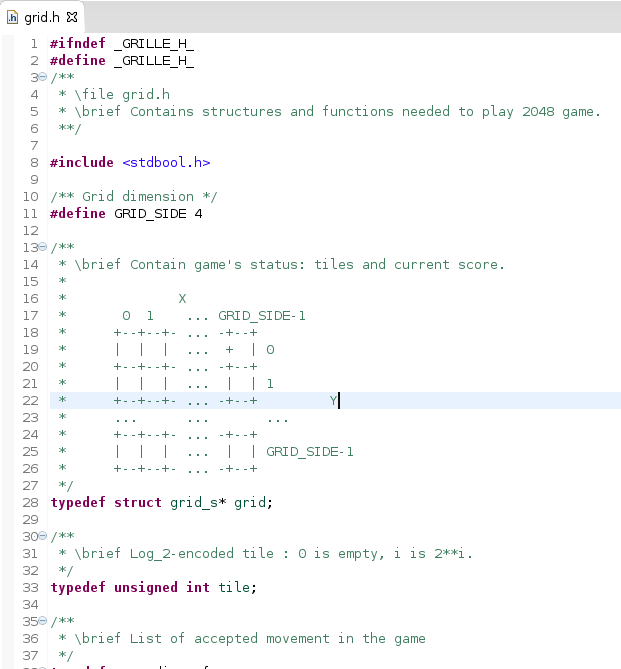
\includegraphics[scale=0.6]{grid_h.png}
\end{figure}

\begin{figure}
   \caption{\label{grille_couleur} Deuxième version d'affichage de la grille}
   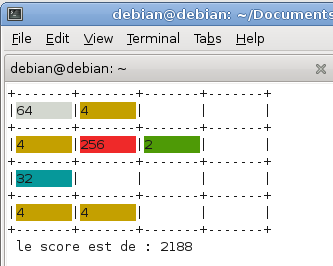
\includegraphics[width=7cm]{grille_couleur.png}
\end{figure}

\begin{figure}
   \caption{\label{test} Résultat exécution des tests}
   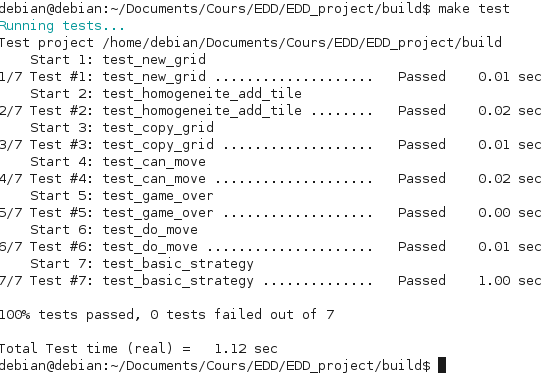
\includegraphics[scale=0.6]{test.png}
\end{figure}

\begin{figure}
   \caption{\label{sdl} Interface graphique avec SDL}
   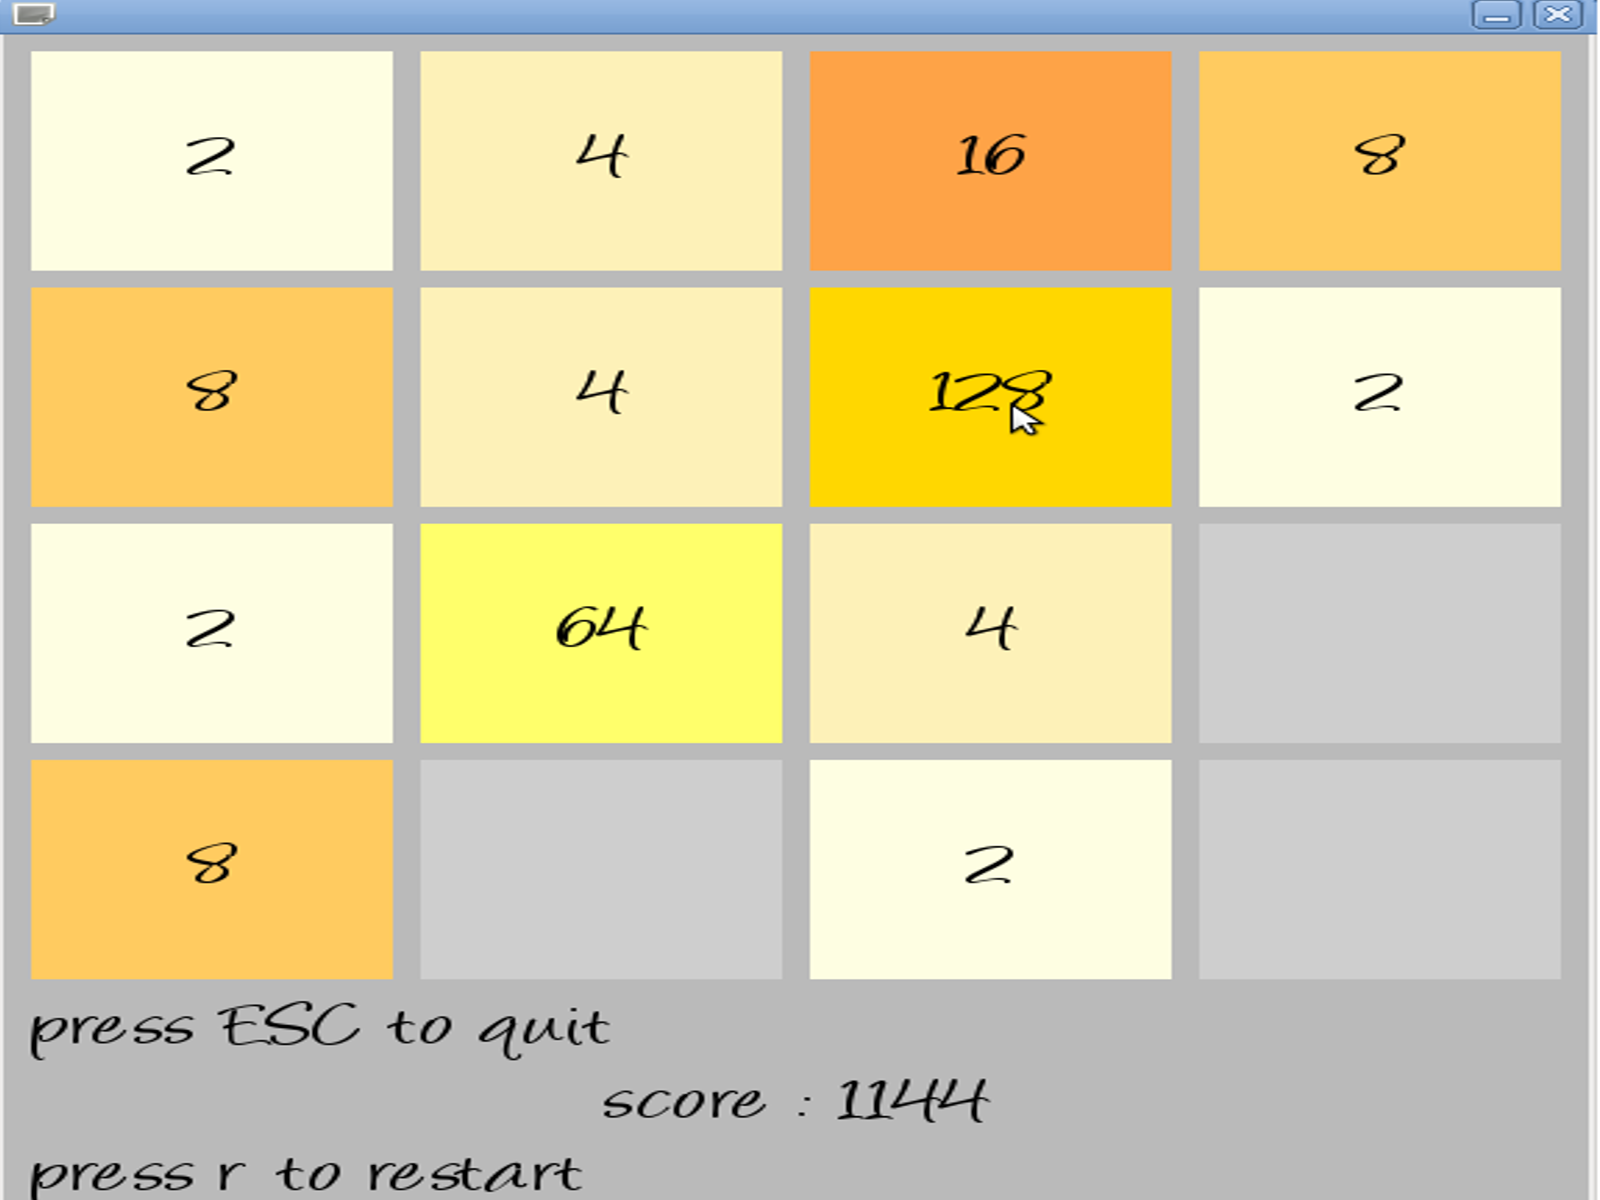
\includegraphics[scale=0.15]{sdl.png}
\end{figure}
\end{document}